\section{Problem 2}

The Matlab files for this exercise are \texttt{multireg.m} and \texttt{hm1\_2.m}

I use the least square loss function to penalize in order to use the gradient function that we have from the slides(slide 9, class3x.pdf).

For the 2-fold cross validation I use the same techinque as the Problem 1, dividing the dataset into 2 sets. I use one set as training and the other as test and vice versa. The plot that is created is far from what we have seen in class. In this exercise I split the dataset in half and not in random. The $\lambda$ that minimizes the testing error is 950 (figure \ref{fig:ex2}).
From the plot we can conclude that the our function that does the penalize does not have underfitting (it is too small).

\begin{figure}[!h]
{
    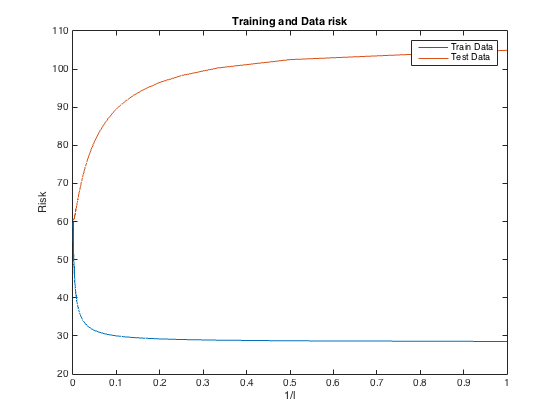
\includegraphics[width=\columnwidth]
    {figures/hm1_2.png}
    \caption{\footnotesize{\bf}Training and Testing Risk}
    \label{fig:ex2}
}
\end{figure} 
